
\chapter{Literature Review}
\label{chap:2}

\section{Related Work}

\subsection{Soft Engg}

 Several studies investigated diabetes data and constructed models to predict diabetes. Equation \ref{eq:1} give

\begin{equation} \label{eq:1}
    y=\sum_i x_i+C^2+\frac{1}{\cos{\theta}}
\end{equation}

Figure \ref{tab:sub} shows bla bla
\begin{table}[ht!]
    \centering
     \caption{Supervised Machine Learning Classifier}
     \vspace{2pt}
    \begin{tabular}{lrp{3in}}
    \hline
        \textbf{hello} & \textit{JU} & Header 2  \\ \hline
         Shamim & KMA & In this step, we will describe some supervised machine learning classifiers namedLogistic Regression, k-nearest neighbors, Support Vector Machine, Decision Tree,Gaussian Naive Bayes, Random Forest, Gradient Boosting and Linear DiscriminantAnalysis. \\  \hline
    \end{tabular}
    \label{tab:sub}
\end{table}

\section{ Machine Learning Types}

\section{Supervised Machine Learning Classifiers}

In this step, we will describe some supervised machine learning classifiers named Logistic Regression, k-nearest neighbors, Support Vector Machine, Decision Tree, Gaussian Naive Bayes, Random Forest, Gradient Boosting and Linear Discriminant Analysis. 

\subsection{Logistic Regression (LR)}

Logistic Regression (LR) is a supervised machine learning data classification algorithm that mines real-valued features from the input, multiplies each of them by a weight, adds them, and transfers the sum through a sigmoid function to produce a probability. A threshold is used to finalize a decision \cite{DSR}. A solution for classification of our data set is LR which Instead of fitting a straight line or hyperplane uses the logistic function to squeeze the output of a linear equation between 0 and 1. The logistic function is defined as:

\[Logistic (\eta) = 1/(1 + exp (-\eta))\]

As $\eta$ goes from $-\infty$ to $\infty$, logistic ($\eta$) goes from 0 to 1, a “squashing function”. In our study, we used a maximum 4000 iterations to converge the output.


\subsection{k-nearest neighbors (KNN) }
 (KNN) is a non-parametric process we used for diabetic data classification. In KNN a data is classified by a majority vote of its neighbors, with the data being allotted to the class most mutual amongst its K nearest neighbors estimated by a distance function. If K = 1, then the data is simply allotted to the class of its nearest neighbor. KNN algorithm is as below : 

\begin{algorithm}
\caption{KNN}
\label{pseudoPSO}
\begin{algorithmic}[1]
\State Let $m$ be the number of training data samples. Let $p$ be an unknown point that needs to be classified
\State Storing the training samples in an array of data points $arr[]$. Each element of this array denotes a tuple $(x, y)$.

\For{$i=0$ to $m$}
    \State Calculating distance $d(arr[i], p)$
   
\EndFor
\State Making set $S$ of $K$ smallest distances achieved. Each of these distances resembles an already classified data point
\State Returning the majority label among $S$
\end{algorithmic}
\end{algorithm}


\subsection{Decision Tree (DT)}
A DT is a classifier that recursively performs partition of the instance space. The decision tree contains nodes that form a tree, a node called “root” that has no incoming edges is the starting point of the tree. All other nodes have one incoming edge. The leaf nodes are known as decision nodes. The child node is nominated by computing Information Gain (IG).

Information Gain = Entropy(parent) - [weights average] * Entropy(children)

Entropy($Ci$) = -P($xi$) log P($xi$), where P($xi$) is the probability of child node $i$. 

Node with the highest IG will be the parent for next level. This process is continued until it gets a leaf node and completed decision tree. 

The algorithm for generating a decision tree is as below :

\begin{algorithm}
\caption{DT}
\label{pseudoPSO1}
\begin{algorithmic}[1]

\State  Create (T) 
\State Calculate frequencies (Ci, T)
\State  If all instances belong to the same class, returning leaf 
\State for every attribute a test is set for splitting criteria. An attribute that satisfies the test is test node K
\State  Repeating Create (Ti) on each partition Ti.Adding those nodes as children of node K

\end{algorithmic}
\end{algorithm}





\subsection{Gaussian Naive Bayes (GNB)}
The GNB classifier is a probability distribution function having the effect of associating neural activation to the means and variances of activation in various impulse conditions. The production of the classifier is a condition-label.  The classifier creates hypothesis that the classes have Gaussian normal distributions.

The z-score distance between the inputted point and each class-mean is estimated for each data point, namely the distance from the class mean divided by the standard deviation of that class.

\begin{equation*}
    Z_A=\frac{(x-\mu_A)}{\sigma_A}
\end{equation*}

According to the equation for a Gaussian normal distribution, each z-score is then converted into a probability value which is used for observing data point x. The co-variance between dimensions is not modelled by GNB classifier.


\subsection{Random Forest (RF)}
RF is a collective algorithm which was modelled from trees algorithm and Bagging algorithm. It works fine with a data set with a large number of input variables. It is a meta estimator that creates a number of decision tree classifiers on different sub-samples of the data set and uses mean value to increase the accuracy of the model and control over-fitting. Suppose training data set is given as: [X1, X2, X3, X4] with labels as [L1, L2, L3, L4] respectively, random forest algorithm may create three decision trees taking input of subset for example, [X1, X3, X4], [X2, X3, X4] and [X1, X2, X4]. Finally, it predicts class based on the majority of votes from each of the decision trees generated. Generally, the more trees in the forest the more robust and reliable the forest is. The random forest classifier works in the same way, the higher the number of trees in the forest gives higher accuracy output .


\subsection{Gradient boosting (GB)}
GB includes three components: a loss function that is to be optimized, a weak learner that makes predictions and an additive model which will add weak learners to minimize the loss function. 









\section{Research Gap}
Analyzing related works in this field an be noticed some shortcoming in the security measurements of IoT network. \textbf{Firstly}, there is no centralized detection method is mentioned, every layer has specific detection way method but as IoT is becoming a heterogenous network a centralized model should be proposed in controller which will control the traffic of every subpart of network. \textbf{Secondly}, by using KDD Dataset most commonly \textbf{DDoS, Probe, U2R, R2L} attack has been detected but with advancing technology intruder can attack the network in many other ways. \textbf{Thirdly}, no time efficient optimal way is mentioned to detect attack. \textbf{Fourthly}, traditional firewall can’t detect any encrypted incoming packet which can be removed by using adaptive firewall concept but still much work has not done yet regarding this problem \cite{mahmud_brain-inspired_2018,8742551,noauthor_coronavirus_nodate}.

\begin{figure}[!htb]
    \centering
    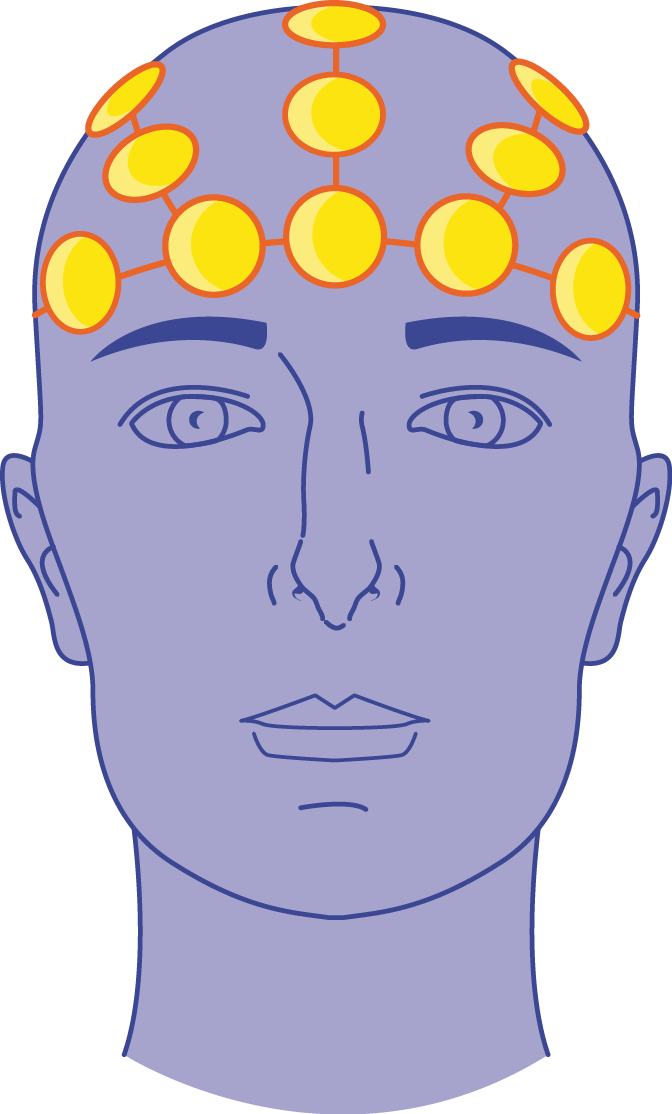
\includegraphics[scale=0.5]{Chap2/EEGonbrain.png}
    \caption{EEG probe on brain}
    \label{fig:my_label}
\end{figure}